\documentclass{article}
\usepackage[polish]{babel}
\usepackage[a4paper, margin=2cm]{geometry}
\usepackage{graphicx}
\usepackage{polski}
\usepackage[utf8]{inputenc}
\usepackage{lettrine}
\usepackage{xcolor}
\usepackage[nodayofweek]{datetime}
\renewcommand{\familydefault}{\sfdefault}

\usepackage[autocite=superscript]{biblatex}
\addbibresource{bibliography.bib}

\title{Historia boulderingu i jego pięć znaczących postaci}
\author{Marcin Młynarczyk}
\newdate{date}{11}{6}{2020}
\date{\displaydate{date}}
\definecolor{blue}{cmyk}{.6,.28,0,.04}

\usepackage{sectsty}
\chapterfont{\color{blue}}
\sectionfont{\color{blue}}
\subsectionfont{\color{blue}}

\addto\captionspolish{
  \renewcommand{\contentsname}%
    {\color{blue}Spis treści}%
}

\begin{document}

\maketitle
\tableofcontents

\bigskip

\begin{figure}[!htbp]
	\begin{center}
		\includegraphics[width=0.7\linewidth]{images/intro.eps}
	\end{center}
	\caption{Roman Batsenko na Gourmandise Raccourci 8A+, \textit{Fontainebleau}, Francja (fot. Karolina Stawoska) \cite{8a}}
\end{figure}

\section{Wstęp}
\lettrine[lines=2]{B}{ouldering} staje się coraz popularniejszą formą aktywności fizycznej. Owy termin, w swojej angielskiej postaci, dość mocno zakorzenił się w polskim żargonie wspinaczkowym. Pojęcie \textit{bouldering} pochodzi z języka angielskiego, w którym oznacza \textit{głaz}. Zatem uprawianie boulderingu to w dosłownym tłumaczeniu "głazowanie", czyli wspinanie się na głazy. W języku polskim można się również spotkać z lekko spolszczoną wersją tego terminu - \textit{baldering}. W dużym uproszczeniu, i trochę żartobliwie, bouldering można zdefiniować jako "wchodzenie na kamyki od trudnej strony". W odróżnieniu od wspinaczki z liną, asekurację najczęściej stanowią tutaj materace rozłożone w potencjalnej strefie upadku. Z tego również powodu, jako obiekt wspinania obiera się tutaj z reguły wolno stojące głazy poniżej 6 m wysokości. Niemniej jednak, można spotkać od tej reguły wyjątki, np. boulder o nazwie \textit{Ambrosia} w Bishop w USA posiada ponad 16 m wysokości \cite{ambrosia}.

\begin{figure}[!htbp]
	\begin{center}
		\includegraphics[width=0.7\linewidth]{images/nina-williams-abrosia.eps}
	\end{center}
	\caption{Nina Williams i słynny highball “Ambrosia” (fot. Nayton Rosales) \cite{nina}}
	\label{ambrosia}
\end{figure}

\section{Historia}
\lettrine[lines=2]{S}{kupię} się na przedstawieniu światowej historii rozwoju omawianego w tej pracy sportu, jako że w dostępnych źródłach bardzo ciężko doszukać się informacji na temat polskiej historii boulderingu. Postaram się przytoczyć okoliczności powstania boulderingu, a następnie przejdę do przedstawienia jego obecnej sytuacji. Wspaniałym źródłem wiedzy o historii boulderingu okazały się materiały \cite{gill-history} napisane przez ojca współczesnego boulderingu - Johna Gill'a - o którym więcej napiszę w sekcji \ref{jg}. W tej pracy, nie jestem w stanie w tak dokładny i ciekawy sposób przekazać dostępnej tam wiedzy, dlatego zaciekawionego czytelnika zachęcam do zapoznania się z owymi materiałami - szczególnie interesującymi są liczne fotografie z przełomu XIX i XX wieku, ukazujące wspinaczy uprawiających czynności jak najbardziej przypominające bouldering (Rysunek \ref{benson}). Bardzo ciekawy opis rozwoju boulderingu, przedstawiający trochę inne aspekty tego procesu i reprezentujący inne spojrzenie od tego przedstawionego poniżej, czytelnik może znaleźć w artykule \cite{pg-hist}.

\begin{figure}[!htbp]
	\begin{center}
		\includegraphics[width=0.5\linewidth]{images/old1.eps}
	\end{center}
	\caption{British Mountaineering, 1909 (fot. Claude E. Benson) \cite{gill-history}}
	\label{benson}
\end{figure}

\subsection{Początki}
Istnieją przypuszczenia, że początki nieudokumentowanego boulderingu sięgają drugiej połowy XIX wieku. Zaczynał wtedy rozkwitać alpinizm i gdy nie dopisywała pogoda, wspinacze mieli ćwiczyć na owych małych głazach jako przygotowanie do późniejszych ekspedycji. Mogliśmy takie praktyki najprawdopodobniej obserwować w m.im. \textit{Fontainebleau} we Francji, czy \textit{Lake District} w Wielkiej Brytanii. Niemniej jednak, takie podejście wspinaczy ukazywało bouldering jako środek do osiągnięcia "wyższych celi" i nie widziało w jego istocie sportu w pełnej okazałości. Ktoś mógłby rozsądnie i dociekliwie zatem zapytać, a z kiedy mamy pierwsze udokumentowane doniesienia o bardziej poważnym podejściu do rozważanej tutaj formy wspinaczki?

Na arenie międzynarodowej, to wspinacz Oscar Eckenstein, pochodzący z Wielkiej Brytanii, wydaje się być prekursorem boulderingu pokazującego oddanie tej dyscyplinie, zbliżone do tej które możemy obserwować w dzisiejszych czasach. Eckenstein żył na przełomie XIX i XX wieku i wspinał się m.in. w rejonie \textit{Lake District}. Aleister Crowley miał rzekomo mówić, że Eckenstein był w stanie pokonać problem na \textit{Y-Boulder} w \textit{Lake District} (rysunek \ref{collier}), którego inni wybitni wspinacze w ówczesnym momencie nie byli w stanie przejść. Zdaniem Johna Gill'a Eckenstein mógł być pierwszym prawdziwym mistrzem tego sportu - był wspinaczem, który nie tylko poszerzał standardy trudności, ale również w dość znaczący sposób przyczyniał się do ewolucji filozofii i praktykowania boulderingu. Niemniej jednak, większość brytyjskich wspinaczy dalej nie dostrzegała w tej formie wspinaczki oddzielnej dyscypliny.

\begin{figure}[!htbp]
	\begin{center}
		\includegraphics[width=0.5\linewidth]{images/y-boulder-collier.eps}
	\end{center}
	\caption{Dr Joseph Collier w trakcie próby przejścia \textit{Y-Boulder}, najprawdopodobniej pokonanej po raz pierwszy przez Oscara Eckensteina. Collier używa "wymaganej" tutaj techniki - próbuje pokonać fragment trasy do góry nogami (fot. George i Ashley Abraham) \cite{gill-history}}
	\label{collier}
\end{figure}

Dopiero w okresie międzywojennym Francuzi zaczęli eksplorować pomysł oddzielenia boulderingu od wspinaczki tradycyjnej, mowa tutaj o Pierre Allain, który wraz ze swoimi towarzyszami popularyzował wspinanie na gigantyczne głazy we francuskim \textit{Fontainebleau} (rysunek \ref{allain-1}). Po drugiej wojnie światowej mieli oni podobno dostrzegać wewnętrzną, nie motywowaną jedynie rozwijaniem umiejętności przydatnych do wypraw wysokogórskich, wartość wspinaczki w tym rejonie (rysunek \ref{allain-2}). Zdaniem Gill'a, Allain również zasługuje na miano mistrza tego jeszcze wtedy raczkującego sportu.

\begin{figure}[!htbp]
	\begin{center}
		\includegraphics[width=0.5\linewidth]{images/allain-1.eps}
	\end{center}
	\caption{Pierre Allain w \textit{Fontainebleau} około roku 1938 (Editions Guerin-Chamoni) \cite{gill-history2}}
	\label{allain-1}
\end{figure}

\begin{figure}[!htbp]
	\begin{center}
		\includegraphics[width=0.35\linewidth]{images/allain-2.eps}
	\end{center}
	\caption{Pierre Allain i Guy Poulet kończący \textit{La Prestat Boulder} w \textit{Fontainebleau}. Po środku Rene Ferlet, a poniżej Jacques Poincenot. Około roku 1948 (Editions Guerin-Chamoni) \cite{gill-history2}}
	\label{allain-2}
\end{figure}

Podobny rozwój boulderingu można było obserwować w Wielkiej Brytanii. Zdaniem Gill'a na Wyspach Brytyjskich bouldering zyskał status zbliżony do obecnego dopiero w ostatniej ćwiartce XX wieku \cite{gill-history-1.2}. Parafrazując przemyślenia Geoffrey'a Winthropa Younga z książki \textit{Mountain Craft (1949)}: \textit{"Wprowadzenie do wspinaczki, którego zazwyczaj doświadczają nowicjusze, polega na ćwiczeniach na pojedynczych skałach, niskich klifach, czy też głazach, z lub bez użycia asekuracji na wędkę. Owy 'bouldering', czy też rozwiązywanie problemów, może służyć odkrywaniu talentu lub zachęcaniu do wspinaczki, ale jest mało użyteczne w trakcie rozpoczynania praktyki [...]"}. W książce \textit{Snowden Biography (1957)} możemy z kolei przeczytać, parafrazując: "\textit{Skały na niższych zboczach i wzgórzach nie były zupełnie brane pod uwagę jako dzień spędzony na prawdziwej wspinaczce. Ćwiczenie boulderingu, takie jak te które wykonywaliśmy w pobliżu naszej bazy, w dni wolne lub mokre, było ograniczonym ćwiczeniem, które niewiele przyczyniało się do poprawy techniki tamtych czasów. Dopiero gdy 'wspinaczkowa gorączka' rozprzestrzeniła się na obszary bez wzgórz, gdzie samotny kawałek żwiru lub piaskowca odgrywał rolę lokalnej góry, tak jak to miało miejsce w Peak District, bouldering, jak to nazywaliśmy, miał szansę rozwinąć się jako praktyka na dużą skalę i produkować swoich ekspertów [...]"} \cite{gill-history-1.2}.

\subsection{Nadejście współczesnego boulderingu}
Współczesny bouldering narodził się w latach 50-tych XX wieku, a za jego ojca można uznać Johna Gill'a (rysunek \ref{gill-1}). W odróżnieniu od wielu wspinaczy jego czasów, Gill szukał we wspinaczce bardziej pochodnej gimnastyki niż pochodnej wędrówki. Zainspirowany gimnastyką artystyczną, mianowicie jej kontrolowanymi ruchami dynamicznymi, zaczął owe ruchy ćwiczyć i wykorzystywać jako technikę pokonywania tras boulderowych. Ponadto, opracował pierwszy oddzielny system wyceny tras dla tej formy wspinaczki, i jak sam przyznaje jest bardzo prawdopodobnym, że był pierwszym w pełni specjalizującym się w boulderingu wspinaczem. Co więcej, starał się od początku promować bouldering jako oddzielny rodzaj wspinaczki, niezależny od konkretnej lokalizacji - w przeciwieństwie do poprzednich starań Pierre Allain'a, aby utożsamić tą formę aktywności z francuskim \textit{Fontainebleau}. Oprócz Gill'a w latach 60-tych w Stanach Zjednoczonych było jeszcze kilku wspinaczy, którzy widzieli w boulderingu samodzielną i autentyczną formę wspinaczki, o których warto tutaj wspomnieć - są nimi: Rich Goldstone, Pat Ament i Pete Cleveland. W latach 70-tych coraz więcej osób zaczęło skupiać swoją uwagę na wspinaniu się na "mniejsze głazy".

\begin{figure}[!htbp]
	\begin{center}
		\includegraphics[width=0.5\linewidth]{images/gill-1.eps}
	\end{center}
	\caption{John Gill, \textit{Red Cross Rock Eliminate, V9}, 1963 \cite{gill-wiki}}
	\label{gill-1}
\end{figure}

W miarę rozwoju sportu, zaczęto dostrzegać ograniczenia skali trudności stworzonej przez Gill'a, była ona bowiem jedynie trójstopniowa. W latach 90-tych John Sherman, o którym więcej w sekcji \ref{js}, zaproponował \textit{V-skalę} jako zamiennik skali Gill'a na użytek w \textit{Hueco Tanks} w Stanach Zjednoczonych. Jako, że okazała się ona bardzo użyteczna, została szeroko przyjęta w Ameryce. W Europie, z kolei, zdominowała skala francuska, pochodząca z \textit{Fontainebleau}. Co ciekawe, na początku współczesnego boulderingu używano okazjonalnego asekurowania na wędkę przy szukaniu rozwiązania problemów. Pod koniec XX wieku, spora większość wspinaczy zrezygnowała z tego sposobu na rzecz materacy i mat boulderingowych.

\subsection{Obecnie}
Największe zmiany jakich bouldering doświadczył od wejścia w okres swojej współczesności dotyczyły pojawienia się licznych krajowych i międzynarodowych zawodów, oraz związanej z tym standaryzacji i wzrostu ustanowionych limitów ludzkich możliwości. John Gill, używając skali z \textit{Hueco}, oszacował i porównał poziom najtrudniejszych tras na przestrzeni historii rozwoju boulderingu \cite{gill-history}. Gill szacuje, że około roku 1900 w Wielkiej Brytanii trudność tras wynosiła ok. V0-V1. Uważa również, że Pierre Allain wraz ze swoimi kompanami dotarł w latach 30-tych XX wieku najprawdopodobniej do poziomu V3, a na przestrzeni kolejnych dwudziestu lat poziom w \textit{Fontainebleau} wzrósł do V4-V5. Poziom trudności swoich tras w późnych latach 50-tych, Gill plasuje pomiędzy V2 i V7, w porywach do V10. Na koniec, Gill stwierdza, że w latach 70-tych, Jim Holloway przekroczył najprawdopodobniej V12. Obecnie, najtrudniejszymi trasami są \textit{Burden of Dreams} i \textit{No Kpote Only} - obie z proponowanym poziomem trudności V17. Ale jak wyobrazić sobie poziom trudności tych tras? Jednym ze sposobów jest uświadomienie sobie ile pracy włożył w przygotowania Nalle Hukkataival - wspinacz który pierwszy, i do tej pory jedyny, przeszedł trasę \textit{Burden of Dreams}. Hukkataival miał podczas tamtego wyczynu na swoim koncie ok. 20 lat wspinaczkowego stażu, a same przygotowania do tej konkretnej trasy - opracowanie sposobu i zdobywanie odpowiedniej siły - zajęły mu ponad 3 lata \cite{hukkataival-yt}. Więcej o tym wspinaczu znajduje się w sekcji \ref{nh}. W zrozumieniu wycen przydatnym może się również okazać porównanie znajdujące się na rysunku \ref{grades}.  

Szczególnie ważnym wydarzeniem dla boulderingu, i dla całego sportu jakim jest wspinaczka, było włączenie tej dyscypliny do Letnich Igrzysk Olimpijskich w roku 2020. Istnieje sporo kontrowersji co do wybranego formatu - każdy wspinacz musi jednocześnie konkurować w trzech, przez wielu uważanych za zupełnie inne, formach wspinaczki: wspinaczce sportowej z dolną asekuracją, boulderingu i wspinaczce na szybkość \cite{olympics}. Zainteresowanemu czytelnikowi może się również spodobać krótki artykuł \cite{great-moments} napisany w języku angielskim, opowiadający o dwunastu wspaniałych momentach w ostatnich dwudziestu latach boulderingu.


\section{Znaczące postaci}
\lettrine[lines=2]{W}{tej} sekcji postaram się przedstawić sylwetki postaci znaczących ze względu na historię rozwoju boulderingu - John Gill, John Sherman i Fred Nicole, oraz sylwetki wspinaczy, którzy obecnie posiadają na swoim koncie najtrudniejsze trasy - wśród mężczyzn Nalle Hukkataival i wśród kobiet Ashima Shiraishi. Przedstawieni tutaj wspinacze nie są w żaden sposób definitywną listą znaczących postaci i dokonany tutaj wybór może nie być najlepszym możliwym - pozwolono sobie na sporo subiektywizmu. Niewykluczone, że bardziej doświadczony od autora czytelnik zupełnie nie zgodzi się z ową selekcją, ale liczę że wybaczy ograniczonej wiedzy twórcy.

\subsection{John Gill}
\label{jg}
O tym bardzo istotnym ze względu na rozwój współczesnego boulderingu wspinaczu niejednokrotnie już w tej pracy wspomniano. Oprócz promowania wydzielenia tej formy wspinaczki jako pełnowartościowego sportu, oraz opublikowania wielu materiałów o historii boulderingu na świecie, przyczynił się on do zaszczepienia w \textit{gimnastycznej odmianie wspinaczki} z goła odmiennej filozofii niż ta obecna w innych formach wspinaczki, szczególnie tych bardziej tradycyjnych. Mianowicie, główna idea, która spodobała się Gill'owi, to minimalizacja obecnego we wspinaczce nieodłącznego ryzyka i skupienie się na zadowoleniu, czy też przyjemności, płynącej ze wspinaczkowego poruszania się, nieskażonego strachem o własne życie \cite{gill-philosophy}. Osobiście, mam wrażenie, że to właśnie przez tą możliwość \textit{po prostu wspinania się}, ową \textit{czystość i prostotę} którą dostrzegł w boulderingu Gill, ta forma znajduje wielu zwolenników. Oczywiście, ryzyko jest w boulderingu dalej obecne i jest on dalej zaliczany jako sport ekstremalny. Szczególnie ryzykownymi wydają się, zaliczane do boulderingu, trasy określane angielskim terminem \textit{highball}, której przykładem może być chociażby wcześniej przytoczona \textit{Ambrosia} (rysunek \ref{ambrosia}).

\begin{figure}[!htbp]
	\begin{center}
		\includegraphics[width=0.5\linewidth]{images/gill-2.eps}
	\end{center}
	\caption{John Gill w wieku 45 lat, 1982 \cite{gill-website}}
	\label{gill-2}
\end{figure}

Gill urodził się w 1937 roku w Stanach Zjednoczonych i zawodowo zajmował się matematyką. Przygodę ze wspinaczką, wówczas tradycyjną, rozpoczął w roku 1953. Po kilku latach zaczął specjalizować się w krótkich trasach, do pokonywania których z wyboru, a czasem z konieczności wykorzystywał dynamiczne ruchy zainspirowane gimnastyką. Warto bowiem, wspomnieć, że Gill był również w młodości gimnastykiem - specjalizował się we wspinaniu po linie i w kółkach gimnastycznych. To właśnie formalny trening gimnastyczny miał być jedną z inspiracji jego podejścia do wspinaczki, mianowicie kładzenie przez niego nacisku na styl i wdzięk sposobu pokonywania boulderów. Gimnastyka sportowa była również motywacją dla Gill'a do rozpoczęcia korzystania z magnezji w boulderingu, co następnie szeroko rozprzestrzeniło się do innych rodzajów wspinaczki \cite{gill-wiki}.

\subsection{John Sherman}
\label{js}
John \textit{Verm} Sherman urodził się w roku 1959 w Stanach Zjednoczonych. Jak już wcześniej zostało wspomniane, opracował \textit{V-skalę}, która początkowo miała służyć lokalnie w \textit{Hueco Tanks}, ale związku z wygodą jej stosowania, m.in. otwartością na poszerzanie jej zakresu w miarę wzrostu umiejętności wspinaczy, rozpowszechniła się na całe Stany. Był główną osobą odpowiedzialną za rozwój \textit{Hueco Tanks}, gdzie przypisuje mu się ponad 400 pierwszych przejść w latach 80-tych i 90-tych XX wieku. Sherman jest również autorem książek o wspinaczce, oraz fotografem \cite{verm-wiki}. W ramach fotografii swoją uwagę szczególnie skupił na uwiecznianiu dzikich ptaków, m.in. zagrożonego wyginięciem kondora kalifornijskiego \cite{vimeo-verm}. 

\begin{figure}[!htbp]
	\begin{center}
		\includegraphics[width=0.5\linewidth]{images/john-sherman.eps}
	\end{center}
	\caption{Najprawdopodobniej najpopularniejsze zdjęcie Johna Shermana, sam Sherman posiada je jako zdjęcie profilowe oficjalnego konta w portalu Facebook \cite{js-photo}}
\end{figure}

Z fotografiami zrobionymi przez Johna Shermana można zapoznać się na jego stronie \cite{vermphoto}. W zakładce \textit{Who the Hell is Verm?} można znaleźć jego krótką i humorystyczną autobiografię. Dla zainteresowanych, tutaj \cite{vermfb} możemy z kolei znaleźć jego oficjalne konto w portalu Facebook. 

\subsection{Fred Nicole}
Frédéric Nicole, lepiej znany jako Fred Nicole, jest profesjonalnym szwajcarskim wspinaczem. Urodził się w roku 1970 w Vevey. Nicole jest znany ze swojego wkładu w rozwój wielu wspinaczkowych rejonów na świecie na przełomie XIX i XX wieku, m.in. \textit{Hueco Tanks} w Texasie, \textit{Bishop} w Kalifornii i \textit{Rocklands} w Południowej Afryce. Najwięcej uwagi poświęcił jednak rozwojowi wspinaczki w Szwajcarii. Na przestrzeni lat zgromadził duży dorobek pierwszych przejść problemów, np. \textit{Boa} V15 w Szwajcarii w roku 2011 czy \textit{Esperanza} V14 w \textit{Hueco Tanks} w roku 2001. Nicole zaczął się wspinać w wieku 13 lat za namową swojego brata François. Co ciekawe, za pierwszym razem Nicole stwierdził, że nie lubi wspinaczki i dopiero kolejne próby w następnych miesiącach sprawiły, że pokochał ten sport. Dość szybko w swojej karierze skupił się w głównej mierze na boulderingu. W roku 1996 zaliczył pierwsze przejście problemu \textit{Radja} w Branson w Szwajcarii. Problem zyskał ocenę V14 - pierwsza trasa, która takową w owym czasie otrzymała. Obszerniejsza lista pierwszych przejść tego wspinacza znajduje się we francuskiej notce biograficznej \cite{wiki-nicole}. Obecnie Nicole zajmuje się projektowaniem obuwia wspinaczkowego \cite{climb-nicole}.

\begin{figure}[!htbp]
	\begin{center}
		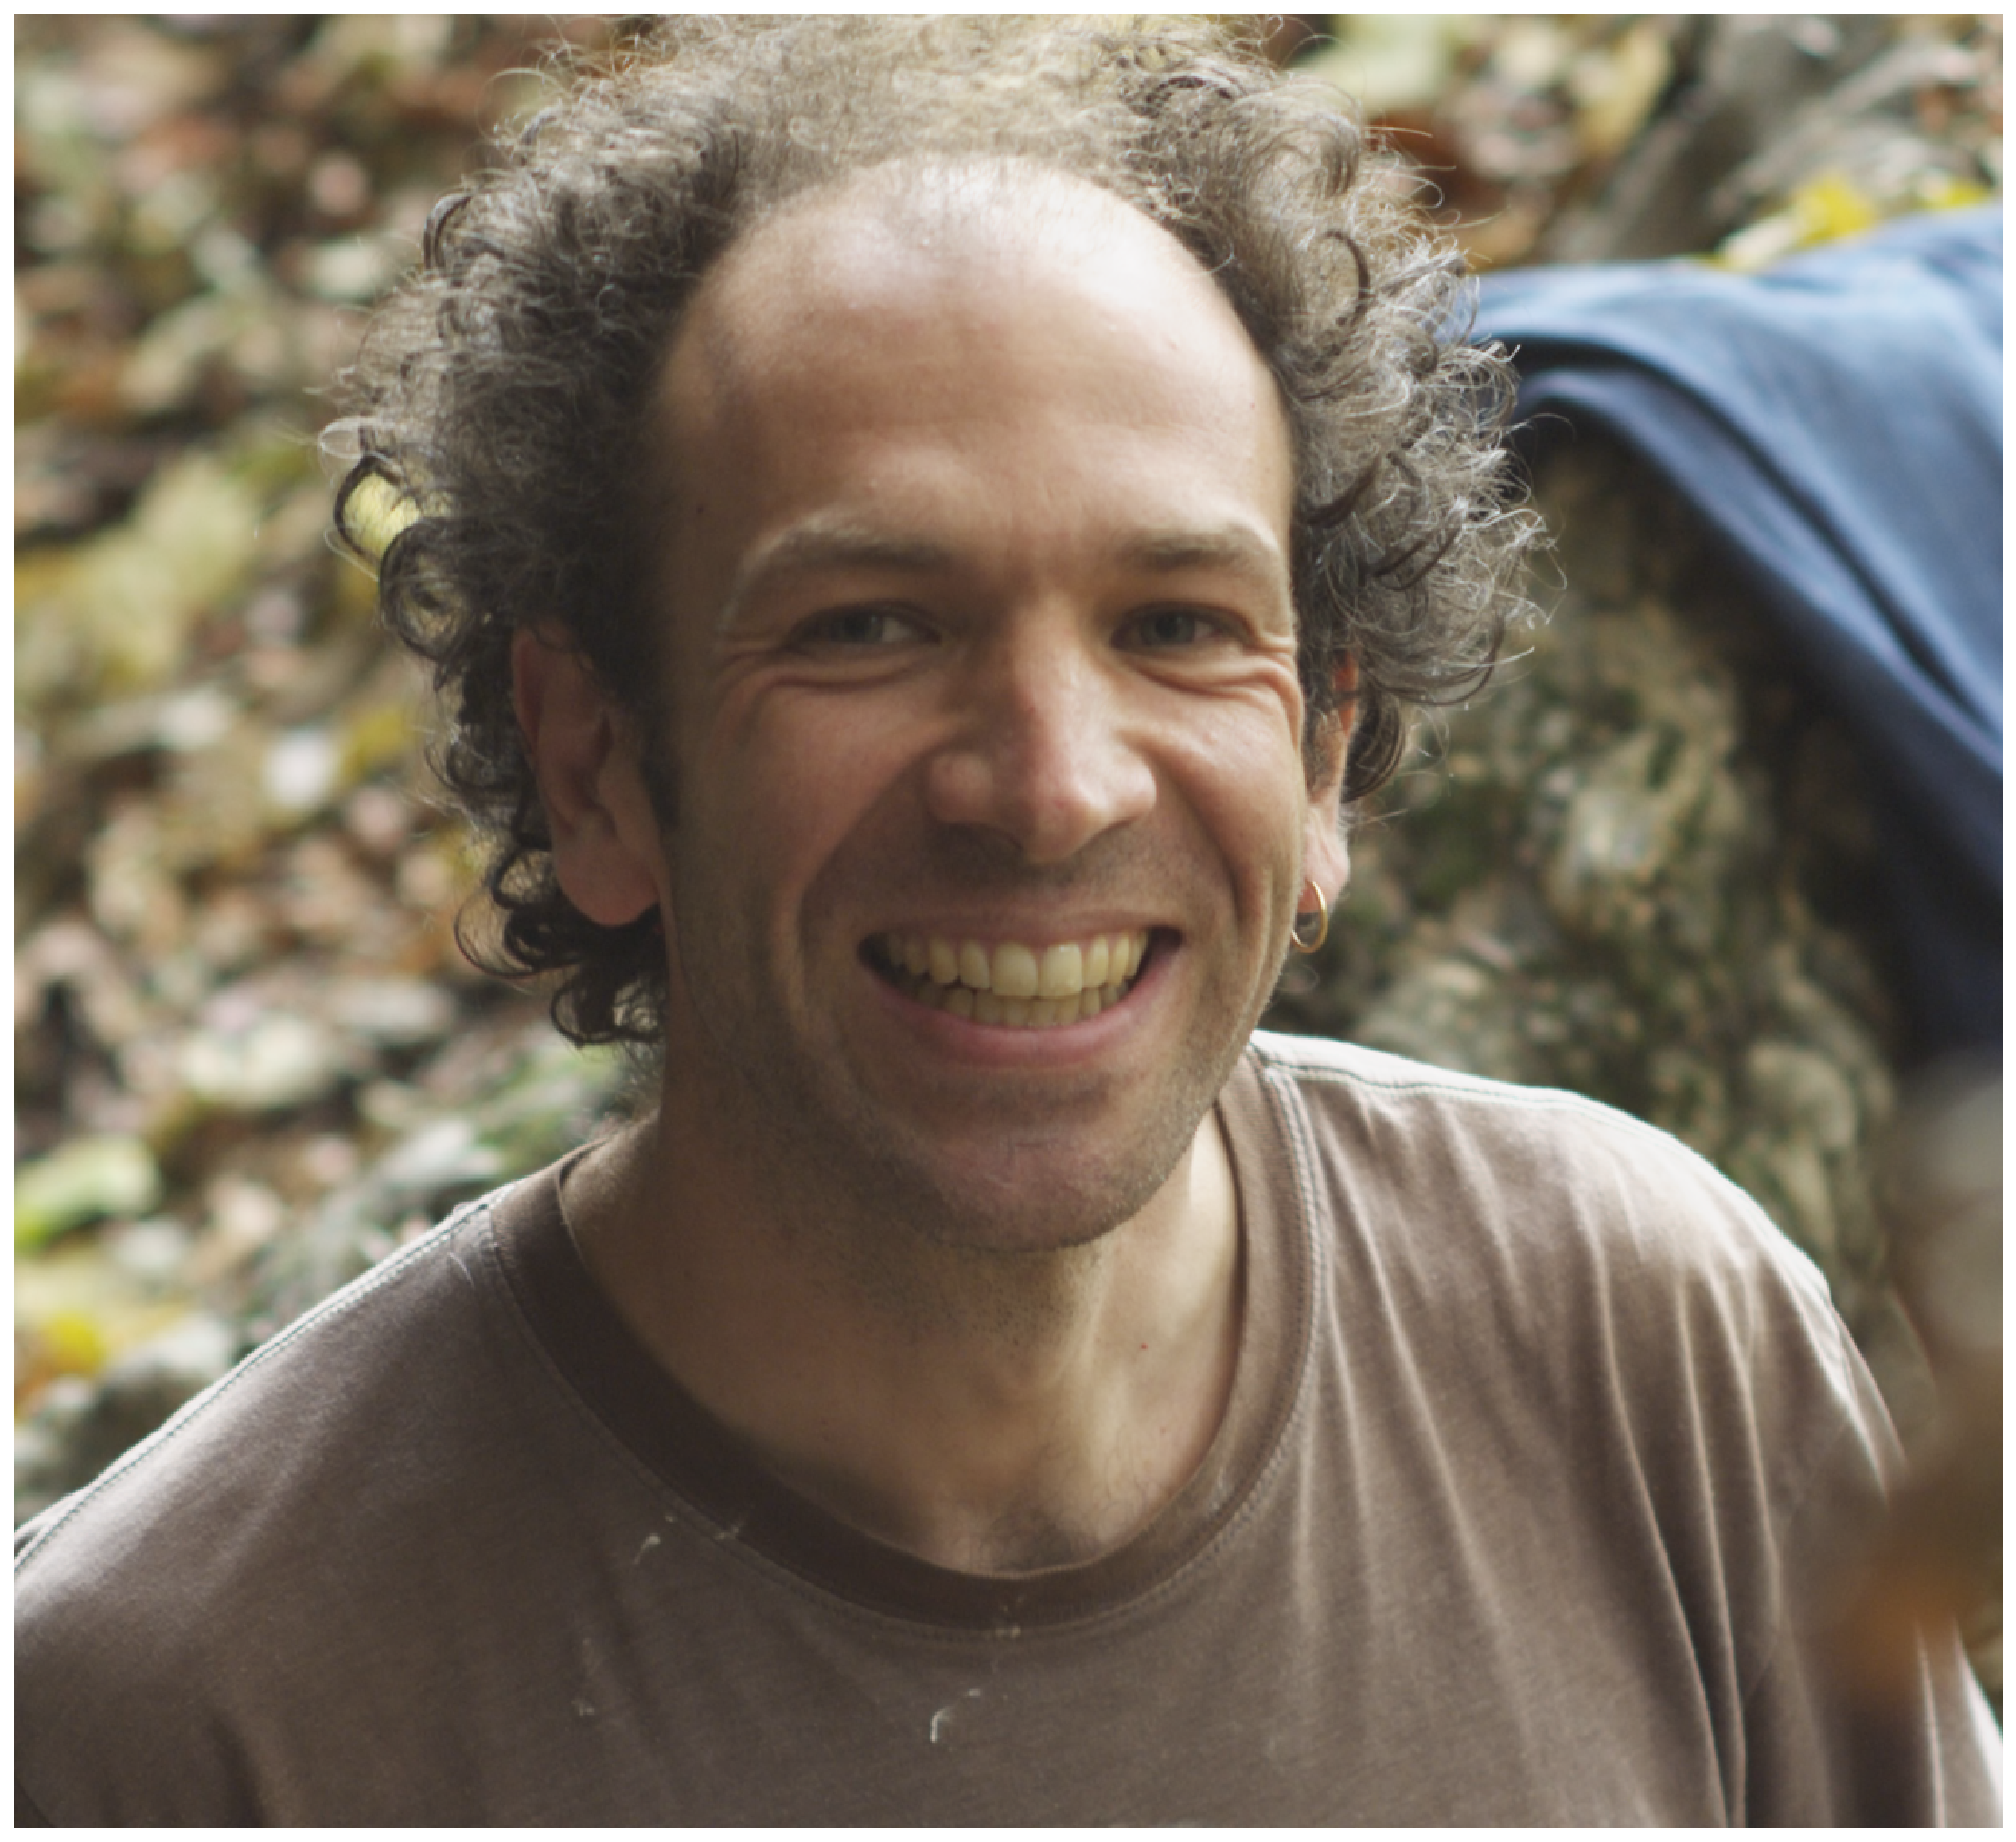
\includegraphics[width=0.5\linewidth]{images/nicole.eps}
	\end{center}
	\caption{Fred Nicole, 2012 \cite{wiki-nicole}}
	\label{nicole}
\end{figure}

\begin{figure}[!htbp]
	\begin{center}
		\includegraphics[width=0.5\linewidth]{images/grades.eps}
	\end{center}
	\caption{Próba porównania \textit{V-skali} i skali francuskiej \textit{Fontainebleau} wraz z podziałem na kategorie zaawansowania \cite{grades}}
	\label{grades}
\end{figure}

\subsection{Ashima Shiraishi}
Ashima Shiraishi jest najmłodszą osobą znajdującą się w tym zestawieniu - urodziła się w 2001 roku w Stanach Zjednoczonych. Przygodę ze wspinaczką rozpoczęła w wieku 6 lat. Jedynie kilka lat później, zapewniła sobie pozycję jednej z najlepszych wspinaczek na świecie w boulderingu i prowadzeniu. W roku 2017 była uważana za najlepszą nastoletnią wspinaczkę obu płci. Jej dorobek składa się z wielu pierwszych miejsc na największych zawodach świata, np. w \textit{Climbing World Championships} i \textit{USA Open Championships}. W roku 2016 została pierwszą kobietą, i najmłodszą osobą - 14 lat, której udało się przejść trasę o wycenie V15. Mowa tutaj o boulderze \textit{Horizon} w Japonii (rysunek \ref{ashima-horizon}). Gdyby powyższy wyczyn nie był wystarczającym, Shiraishi ma na swoim koncie co najmniej trzy problemy o wycenie V14 i co najmniej dziesięć o wycenie V13 \cite{wiki-ashima}. Dodatkowo, warto wspomnieć, że cały powyższy dorobek zdobyła przed 16-tym rokiem życia. Nagrano o niej kilka dokumentów. Najnowszym z nich jest \textit{Obe And Ashima} z roku 2017. Jej obecne poczynania można śledzić w portalu Facebook \cite{ashima-fb} i Instagram \cite{ashima-ig}.

\begin{figure}[!htbp]
	\begin{center}
		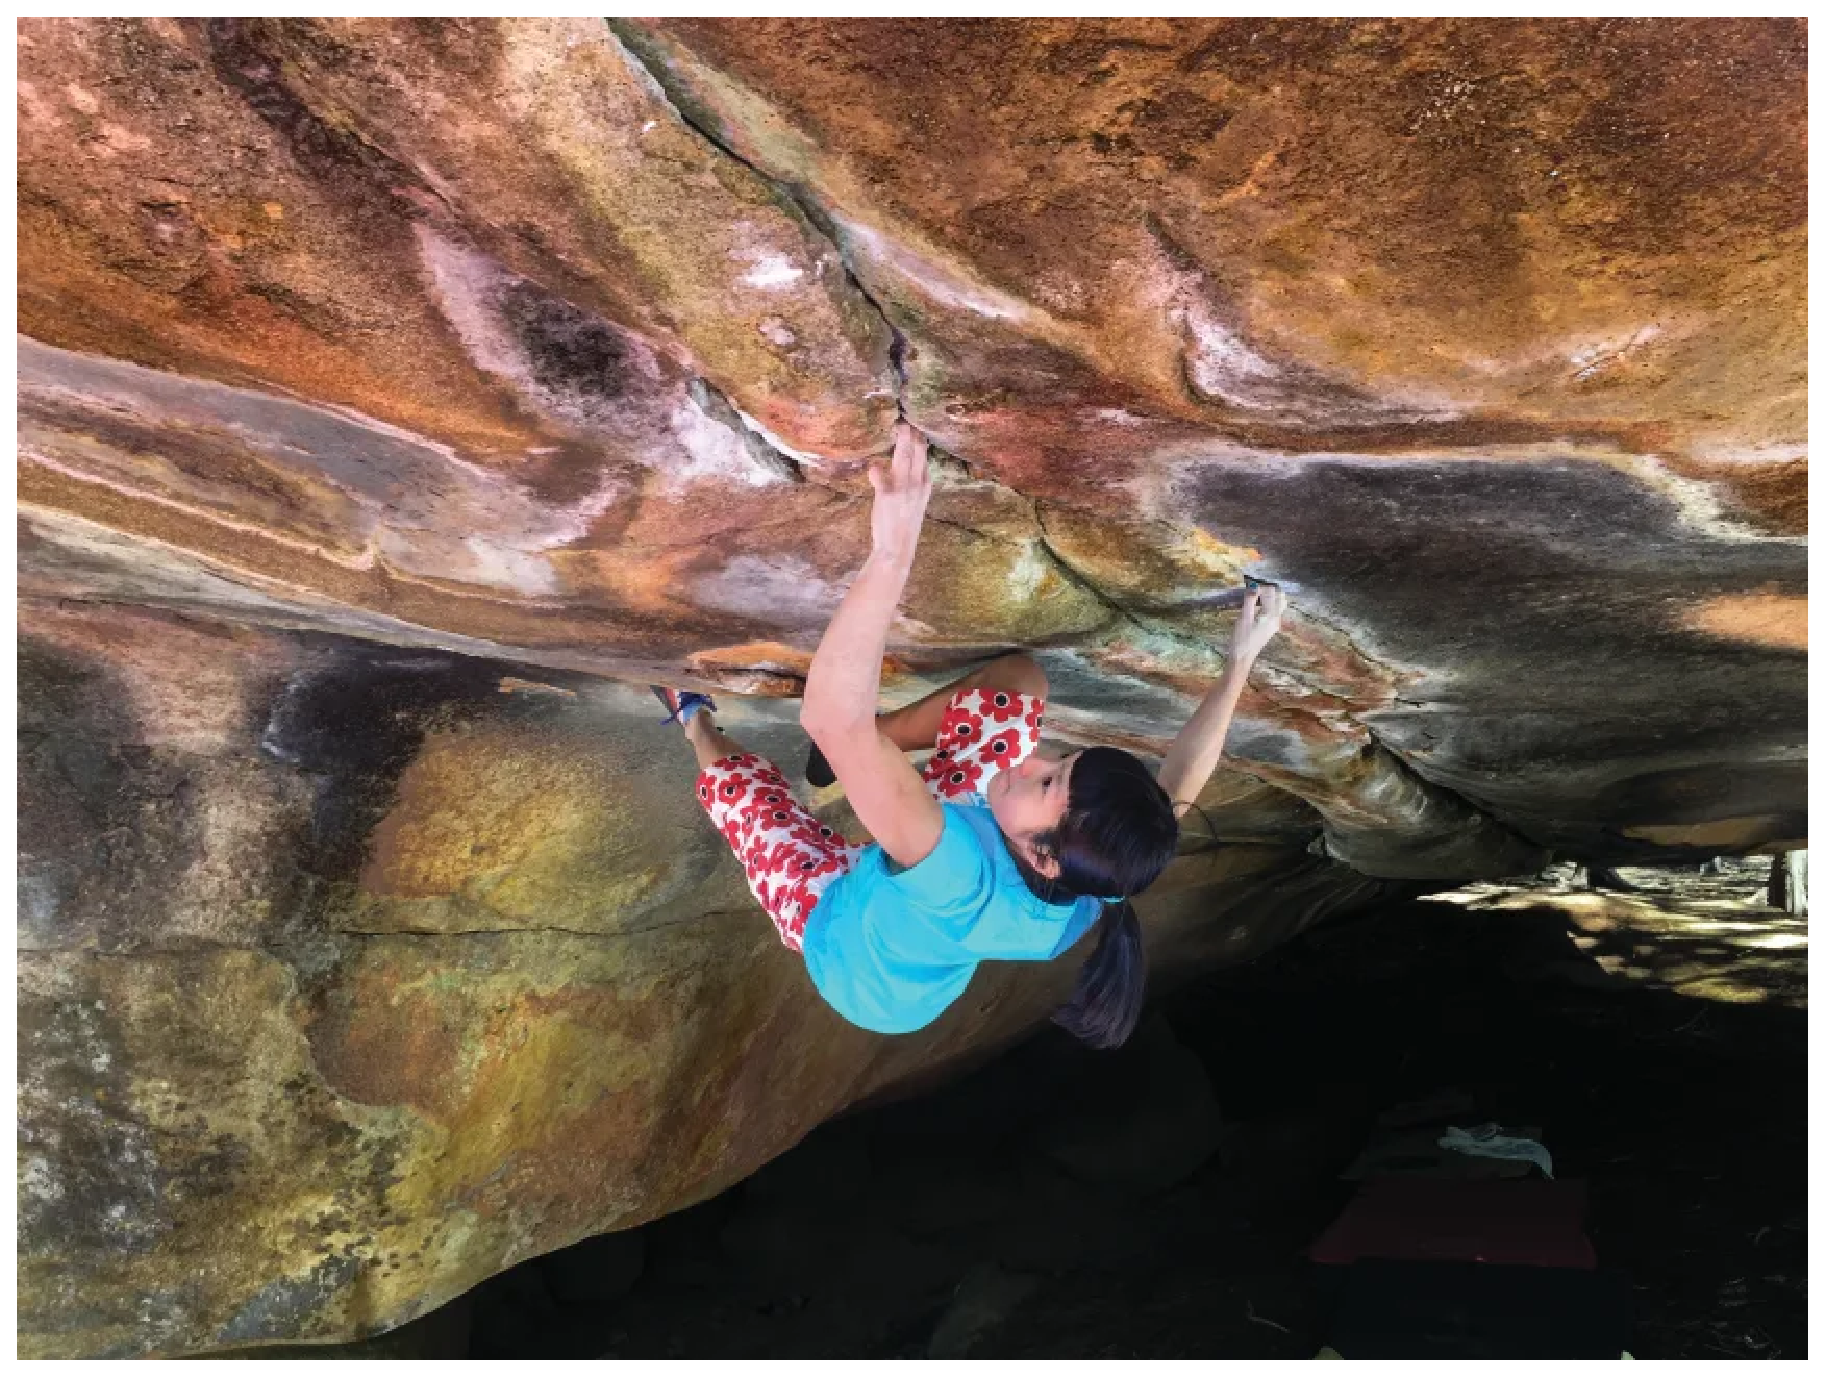
\includegraphics[width=0.6\linewidth]{images/ashima.eps}
	\end{center}
	\caption{Ashima Shiraishi w trakcie pokonywania \textit{Horizon} V15, Japonia, 2016 (fot. Brett Lowell) \cite{climb-ashima}}
	\label{ashima-horizon}
\end{figure}

\subsection{Nalle Hukkataival}
\label{nh}
O Nalle Hukkataival wspomniano już w tej pracy przy omawianiu obecnie najtrudniejszych wytyczonych tras w boulderingu. Hukkataival urodził się w roku 1986 w Helsinkach w Finlandii. Jest profesjonalnym wspinaczem, który specjalizuje się w boulderingu. W swoim dorobku ma wiele pierwszych przejść tras o trudnościach V15, np. \textit{Kintsugi} w Red Rocks w stanie Nevada \cite{kintsugi} i V16, np. \textit{The Finnish Line} w Rocklands w Afryce \cite{finnish-line} (obecnie ta trasa może mieć obniżony poziom trudności do V15 - ciekawe spojrzenie na problematykę wyceny tras można przeczytać w artykule \cite{climb-hukka} napisanym w języku angielskim). Większość boulderów, które udało mu się pokonać, o trudności równej co najmniej V15 możemy znaleźć w artykule \cite{hardest}. Ponadto, jest 4-krotnym zwycięzcą tytułu \textit{Nordic Champion} i 8-krotnym zwycięzcą tytułu \textit{Finnish Champion} w boulderingu \cite{wiki-hukka}. Hukkataival swoją przygodę ze wspinaczką rozpoczął mając 12 lat, a w wieku 17 lat brał udział w swoich pierwszych zawodach.  

O projekcie \textit{Lappnor}, który zaowocował ustanowieniem trasy \textit{Burden of Dreams} o pierwszym na świecie poziomie trudności równym V17, nakręcono nagradzany na festiwalach górskich dokument \cite{docu-lappnor}. Bieżące projekty i poczynania tego wspinacza można śledzić w portalu Facebook \cite{hukka-fb} i Instagram \cite{hukka-ig}.

\pagebreak
\begin{figure}[!htbp]
	\begin{center}
		\includegraphics[width=0.9\linewidth]{images/hukkataival.eps}
	\end{center}
	\caption{Nalle Hukkataival na pierwszym na świecie boulderze o zaproponowanej trudności V17: \textit{Burden of Dreams}, Lappnor, Finlandia. (fot. Nico Backstrom) \cite{climb-hukka}}
	\label{hukka}
\end{figure}

\nocite{*}
\addcontentsline{toc}{section}{Bibliografia}
\printbibliography

\end{document}
